% NETS \& SURFACE AREA - WORKSHEET 0
\documentclass[12pt, letterpaper, fleqn]{article}

% ----------------------------------------------------------
% PACKAGES
% ----------------------------------------------------------
\usepackage{graphicx}
\usepackage{xcolor}
\usepackage[most]{tcolorbox}
\usepackage{amsmath, amssymb}
\usepackage{fancyhdr}
\usepackage[utf8]{inputenc}
\usepackage[T1]{fontenc}
\usepackage{enumitem}
\usepackage{geometry}
\usepackage{tikz}
\usepackage{needspace}
\usepackage{multicol}

\usetikzlibrary{arrows.meta, calc}

% ----------------------------------------------------------
% PAGE SETUP
% ----------------------------------------------------------
\usepackage{times}
\geometry{letterpaper, top=1.25in, bottom=1.25in, marginpar=0.5in}

% ----------------------------------------------------------
% HEADER / FOOTER
% ----------------------------------------------------------
\newcommand{\logowidth}{3cm}
\setlength{\headheight}{20pt}
\setlength{\footskip}{40pt}

\pagestyle{fancy}
\fancyhf{}
\fancyhead[C]{\small\bfseries Nets \& Surface Area}
\fancyfoot[L]{\raisebox{2pt}{
\includegraphics[width=\logowidth]{kss.png}}}
\fancyfoot[C]{\thepage}
\fancyfoot[R]{6.19.0}

\renewcommand{\footrulewidth}{0.2pt}

% ----------------------------------------------------------
% HELPER MACROS
% ----------------------------------------------------------
\newcommand{\blank}{\underline{\hspace{2.2cm}}}
\newcommand{\blanklong}{\underline{\hspace{6.5cm}}}
\newcommand{\blankshorter}{\underline{\hspace{1.5cm}}}

% ----------------------------------------------------------
% DOCUMENT
% ----------------------------------------------------------
\begin{document}


% ==========================================================
% WORKSHEET 0: FOUNDATION
% ==========================================================
\pagestyle{fancy}
\fancyhf{}
\fancyhead[C]{\small\bfseries Nets \& Surface Area --- Worksheet 0}
\fancyfoot[C]{\thepage}
\fancyfoot[R]{6.19.0}
\renewcommand{\footrulewidth}{0.2pt}

\textbf{Name:} \underline{\hspace{5cm}} \hfill \textbf{Date:} \underline{\hspace{3cm}}\\

\begin{tcolorbox}[colback=black!10]
    \large\textcolor{black}{\textbf{Nets and Surface Area (Foundation)}}
\end{tcolorbox}

\vspace{2mm}
\noindent
1. \textbf{Net:} A flattened 2D pattern of polygons that can be folded along its shared edges to construct a closed 3D solid spatial figure.\\
2. \textbf{Surface Area ($SA$):} The total sum of the individual mathematical areas of all two-dimensional faces bounding a 3D solid shape.\\
- \textbf{Rectangular Prism:} Composed of 6 rectangular faces arranged in 3 parallel, congruent pairs: $SA = 2(lw + lh + wh)$.\\
- \textbf{Triangular Prism:} Composed of 2 parallel triangular base plates and 3 rectangular lateral faces matching the base perimeters.\\
- \textbf{Square Pyramid:} Composed of 1 flat square base plate and 4 symmetrical lateral triangular faces meeting at a common apex point.

\vspace{3mm}

% --- 2D NET TO 3D PROJECTION SCAFFOLD ---
\begin{center}
\begin{tikzpicture}[scale=0.85, every node/.style={transform shape}]
    % Draw Unfolded Net (Left Side)
    \draw[thick, black, fill=black!5] (0,0) rectangle (2,1.5); % Back
    \draw[thick, black, fill=black!5] (0,1.5) rectangle (2,2.5); % Top
    \draw[thick, black, fill=black!5] (0,-1) rectangle (2,0); % Bottom
    \draw[thick, black, fill=black!5] (0,-2.5) rectangle (2,-1); % Front
    \draw[thick, black, fill=black!5] (-1.5,0) rectangle (0,1.5); % Left Flap
    \draw[thick, black, fill=black!5] (2,0) rectangle (3.5,1.5); % Right Flap
    
    % Net Annotations
    \node at (1,0.75) {\small Back};
    \node at (1,2) {\small Top};
    \node at (1,-0.5) {\small Btm};
    \node at (1,-1.75) {\small Front};
    \node at (-0.75,0.75) {\small Left};
    \node at (2.75,0.75) {\small Right};
    \node[below, black] at (1,-2.6) {2D Unfolded Net Pattern};

    % Arrow Vector
    \draw[->, ultra thick, gray, line width=3pt] (4.5,0) -- (6,0);

    % Draw Folded 3D Prism (Right Side)
    \begin{scope}[shift={(7,-0.5)}]
        \draw[thick, black, fill=black!5] (0,0) rectangle (2,1.5); % Front
        \draw[thick, black, fill=black!5] (2,0) -- (2.8,0.6) -- (2.8,2.1) -- (2,1.5) -- cycle; % Right side
        \draw[thick, black, fill=black!5] (0,1.5) -- (0.8,2.1) -- (2.8,2.1) -- (2,1.5) -- cycle; % Top Side
        \node at (1,0.75) {\small Front};
        \node at (2.4,0.9) {\small Right};
        \node at (1.4,1.8) {\small Top};
        \node[below, black] at (1.4,-0.6) {3D Folded Solid Figure};
    \end{scope}
\end{tikzpicture}
\end{center}

\vspace{2mm}

\begin{tcolorbox}[colback=white, colframe=black!25, boxrule=0.6pt, arc=4mm, left=6mm, right=6mm, top=4mm, bottom=4mm]
\textbf{Worked Example: Square Pyramid Surface Area}

\medskip
\noindent
Find the surface area of a square pyramid where the square base has side lengths of 5 cm, and the lateral triangles have a slant height ($l$) of 6 cm.\\
\textbf{Solution:}\\
1) $\text{Base Area } (B) = s^2 = 5\text{ cm} \times 5\text{ cm} = 25\text{ cm}^2$.\\
2) $\text{Area of Four Triangles} = 4 \times \left(\frac{1}{2} \cdot b \cdot h_{slant}\right) = 4 \times \left(\frac{1}{2} \cdot 5 \cdot 6\right) = 4 \times 15 = 60\text{ cm}^2$.\\
3) $\text{Total Surface Area } (SA) = \text{Base Area} + \text{Lateral Area} = 25 + 60 = 85\text{ cm}^2$.
\end{tcolorbox}

\newpage

\begin{tcolorbox}[colback=white, colframe=black, boxrule=1pt, arc=4mm, left=6mm, right=6mm, top=5mm, bottom=5mm]
\textbf{Deeper Thinking Problem 1: Triangular Prism Decomposition}

\medskip
\noindent
\textbf{a)} A triangular prism has a right-triangular base with edge sides measuring 3 in, 4 in, and 5 in. The interior height length connecting both bases spans exactly 6 in. Sketch a flat 2D net layout pattern representation of this spatial solid figure below and cleanly label all physical dimensions.
\vspace{7cm}

\noindent
\textbf{b)} Calculate the absolute total surface area of this specific triangular prism using your net model. Detail your work steps clearly for each of the 5 individual bounding polygonal faces.
\vspace{8cm}
\end{tcolorbox}

\vspace{4mm}

\begin{tcolorbox}[colback=white, colframe=black, boxrule=1pt, arc=4mm, left=6mm, right=6mm, top=5mm, bottom=5mm]
\textbf{Deeper Thinking Problem 2: Surface Area vs. Volumetric Ratios}

\medskip
\noindent
\textbf{a)} Two distinct shipping blocks hold an identical net volume capacity of 8 cubic feet. Block A is a cube measuring $2 \times 2 \times 2$ feet. Block B is a flat container measuring $1 \times 2 \times 4$ feet. Compute the complete surface area profiles of both boxes. Which form utilizes less structural raw material?
\vspace{7cm}

\noindent
\textbf{b)} If a symmetric cube displays an absolute outer surface area calculation of 96 square inches, deduce the surface area of one isolated square base face, determine its core edge side length, and calculate its complete spatial capacity volume.
\vspace{8cm}
\end{tcolorbox}

\newpage

\begin{tcolorbox}[colback=white, colframe=black, boxrule=1pt, arc=4mm, left=6mm, right=6mm, top=5mm, bottom=5mm]
\textbf{Deeper Thinking Problem 3: Pyramid Topologies}

\medskip
\noindent
\textbf{a)} A regular square pyramid features a base edge line measuring 8 cm and an inclined slant height tracing line of 10 cm. Find the total surface area parameter. Show the mathematical calculation steps for the baseline plate and the lateral perimeter triangles separately.
\vspace{4cm}

\noindent
\textbf{b)} A camping structure model features the geometric design of a symmetric triangular prism with equilateral triangle bases. Each base edge line spans 2 meters and the vertical altitude line of each triangle measures $\sqrt{3}$ meters. The length axis spans 4 meters. Calculate the absolute total fabric area metrics needed to construct all faces.
\vspace{5cm}

\noindent
\textbf{c)} A storage parcel package has dimensions measuring $12\text{ cm} \times 8\text{ cm} \times 5\text{ cm}$. How many net square centimeters of protective plastic sheeting wrapper material are required to insulate the configuration entirely?
\vspace{5cm}
\end{tcolorbox}

\vspace{4mm}

\begin{tcolorbox}[colback=white, colframe=black, boxrule=1pt, arc=4mm, left=6mm, right=6mm, top=5mm, bottom=5mm]
\textbf{Deeper Thinking Problem 4: Real-World Material Optimizations}

\medskip
\noindent
\textbf{a)} A processing factory designs beverage cartons shaped like triangular prisms. The triangular face profile shows a flat baseline of 6 cm and an internal height line of 5 cm. The structural container body extends axially for 20 cm. The remaining two rectangular wall panels each measure $6.5\text{ cm} \times 20\text{ cm}$. Compute the material area for one unit.
\vspace{8cm}

\noindent
\textbf{b)} A robust storage container shows physical parameters measuring 3 ft $\times$ 2 ft $\times$ 2 ft. An engineer intends to coat all 6 exterior bounding walls with enamel paint. If a small canister can cover exactly 10 square feet of surface, isolate the number of cans required.
\vspace{8cm}
\end{tcolorbox}

\end{document}
\end{document}
